% Please do not change the document class
\documentclass{scrartcl}

% Please do not change these packages
\usepackage[hidelinks]{hyperref}
\usepackage[none]{hyphenat}
\usepackage{setspace}
\doublespace

% You may add additional packages here
\usepackage{amsmath}
\usepackage{graphicx}
\usepackage{url}
\usepackage[autostyle]{csquotes}

% Please include a clear, concise, and descriptive title
\title
{
A guide to input methods when considering portability to mobile devices.
}

% Please do not change the subtitle
\subtitle{COMP160 - Software Engineering Essay}

% Please put your student number in the author field
\author{Student number: 1607539}

\begin{document}

\maketitle

\blockquote{
In an interview with Satoru Iwata on the Wii launch website, Akio Ikeda, who was responsible for the accelerometer hardware on the Wii, said ``Of course, when playing a game, the nearest thing to the player is the controller. The controller should therefore be regarded as an extension of the player rather than as part of the console. I always bear in mind the importance of the fact that the player will have far more contact with the controller and UI than the console itself.'' While these comments were obviously made in relation to a console, the importance of interface is particularly relevant to mobile phones \cite {gilbertson2008using}.
}

\section*{Introduction}

The market for mobile games is both lucrative and in growth.  Sensible console and PC game developers will consider the portability of their software to phones and tablets. This will quantitatively include; input methods, output capability, software compatibility, hardware limitations, and qualitatively; whether the games style 
is suitable for a mobile device.  This essay will examine the input methods and limitations of mobile devices, examine three games that have been ported from a console or PC to a mobile device, and propose a methodology to govern effective input design.

\section*{Proper Portability Practices}

Given the dominance of the x86 architecture, common application programming interfaces (APIs) through widely used software like DirectX, and industry standard hardware: high definition monitors, qwerty keyboards, and twin stick console controllers, porting software between like machines can be cheap.  However, with the market for mobile games worth nearly a quarter (\pounds995.1 million) of the entire UK games industry in 2016 \cite {UKIE2017}, console and PC game developers must consider allowing and easing portability to a mobile system.  Bioshock, Grand Theft Auto (GTA), and Final Fantasy (FF) series can be examined as highly successful games that have been ported to smartphones and tablets.

As with many other proper programming practices, allowing flexibility with the hardware input of a game must be considered from the start.  Most game building engines, including Unity and Epic, offer input mappings so that custom events can be created and then later mapped to controls.  This is essential 
to the process of porting a game to another system whose control scheme is different, the software will obviously not automatically translate a keyboard's space bar 
press into a console controller's jump input, but were a jump event defined in the upper levels of the program, a developer can assign that event to any number of different inputs.  This also encourages a level of abstraction when developing a controller program which separates the events from the processes.  It is important to note that if no such input event customisation options are available, in PyGame for example, then one should be created, through a dictionary structure or similar.

\section*{Touch Input}

While console conventions have led to hands and fingers assimilated to 16-button, dual analog console gamepads \cite{parisi2015counterrevolution}, smartphones and tablets can only be relied to have a touchscreen in common.  Any buttons are proprietary and are used to change the volume or lock the device.  A state machine that interprets touch on a touchscreen can have five different states; started, ended, moved, stationary, or cancelled (for instance, if a call were received on a smartphone mid game) and the developer must recreate complex and intuitive controls using some amount of simultaneous touch states.  Accuracy is debatable as a single finger's touch can cover hundreds of pixels \cite{schmidt2010phonetouch}.  All three of the studied games relied upon a virtual joystick for movement mapped to the touch input on the lower left of the screen.  It is an obvious solution given the standard controller convention, and that input mappings exist for joystick axis and amounts.  Game developers must consider whether their control scheme can be replicated on a touch device, if it must be rewritten, or how the game can be balanced if either is inadequate.  While this may work fine for the slow paced FF franchise; Bioshock and GTA rely on precision and reflexes.  GTA has made some attempt to patch this inaccuracy with an enemy lock on and location specific pop up interfaces.  FF makes little effort to adapt a control interface, merely replicating a console controller as an overlay.  Although this may be to promote nostalgia.\\

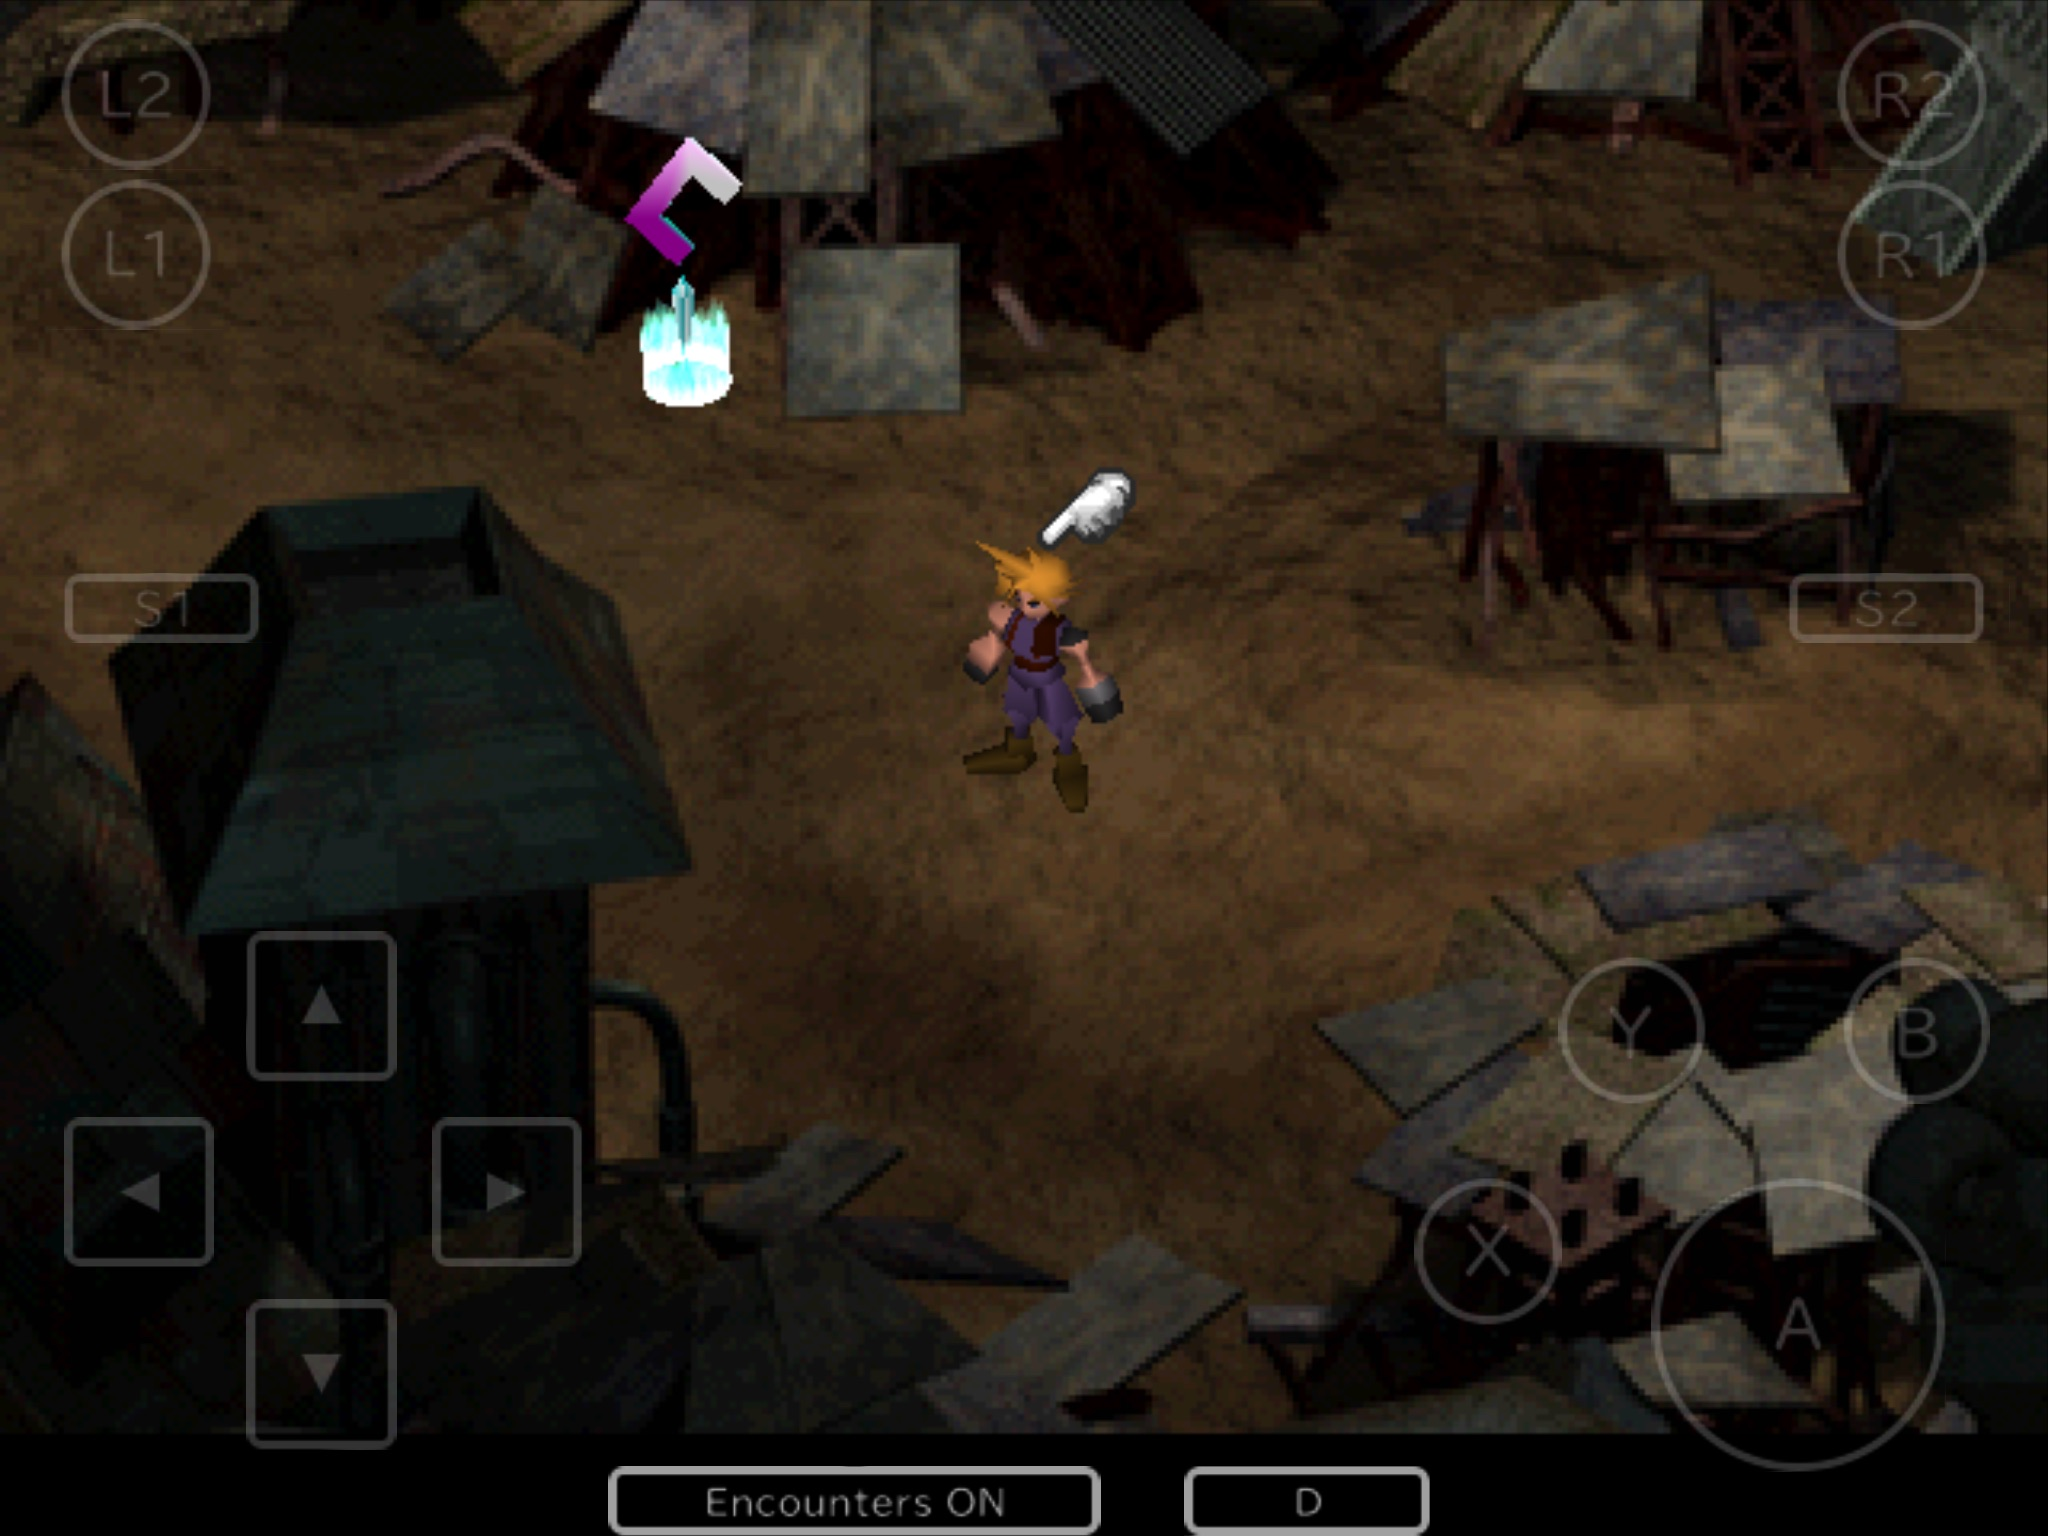
\includegraphics[scale = 0.17]{FF7_IOS_Controls}\\
{
    \emph{Final Fantasy VII} on IOS, on screen controls mimicking a console's controls.
}\\


When touch screen controls are being used, then nothing critical to the player experience should be placed on screen in that space.  GTA mimics police car chases by showing the chasing car appear into the lower left or right portion of the screen.  On a smartphone, this is where the player's hands must be to move the virtual joystick so the experience suffers.  \\

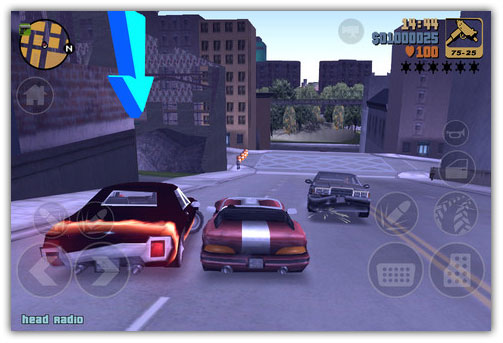
\includegraphics[scale = 0.7]{GTA_IOS_Controls}\\
{
    \emph{Grand Theft Auto III} showing how controls can hide potentially important areas of the screen.
}\\

Bioshock, like all first person shooters (FPS), concentrates the action around the crosshair in the middle of the screen, so controls around the edge are 
more acceptable.  \\

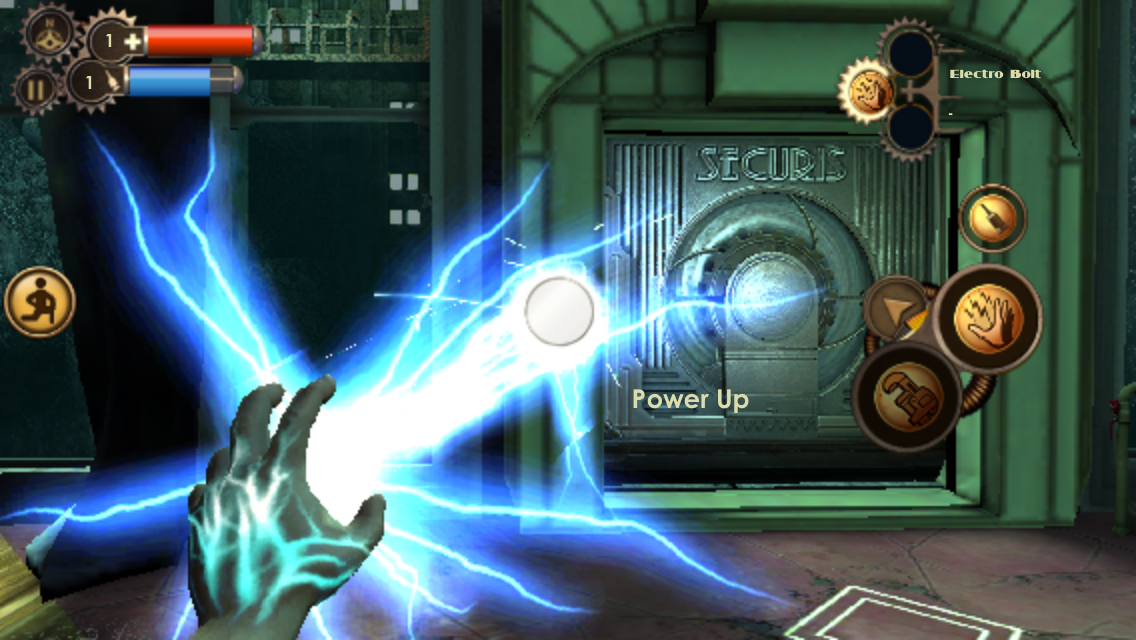
\includegraphics[scale = 0.3]{Bioshock_IOS_Plasmid}\\
{
    \emph{Bioshock} on IOS, plasmids.
}\\

\section*{What are the alternatives?}

Different touchstate types \cite{herz2010multi} are being continually patented which look to add further options to developers.  A good gaming experience requires a lot from the user interface (UI).  It should be convenient, reliable, and usable so that the player can concentrate on playing the game instead of struggling with the UI \cite {korhonen2006playability}.  Hardware abstractions facilitate the ability to play a game on different systems \cite{binsubaih2007survey} but when the control hardware interferes with the UI, alternatives should be considered.  Tilt \cite{gilbertson2008using}, cameras, microphones, gestures \cite{niezen2008gesture}, magnetic tags, accelerometers \cite{harrison2009abracadabra}, and scroll \cite{ballagas2006smart} all serve to remove a player's hands from the play area as much as possible.  An add on controller can be most effective although this incurs extra cost and size to the hardware, although front isometric joysticks are still preferred over a backmounted joystick \cite{wobbrock2007alternative} on a modified device to save size.

As a last resort, the game can be made easier to balance the frustration of missed information, but this is a workaround, not a meaningful solution.

\section*{Conclusion}

The workflow should begin by examining where the important in game information is being shown, then to design any on screen controls around this.  The controls should be intuitive, usually but not always optimally achieved by mirroring the original controller conventions.  Players cannot be expected to always see information under the control interface, and should not be punished for not doing so.  If there is no area of the screen that is not being used then the developer must create some by shifting the player's perspective, being mindful of the smaller screen, or explore non touch alternatives such as tilt controls. 

\bibliographystyle{ieeetran}
\bibliography{references}

\end{document}







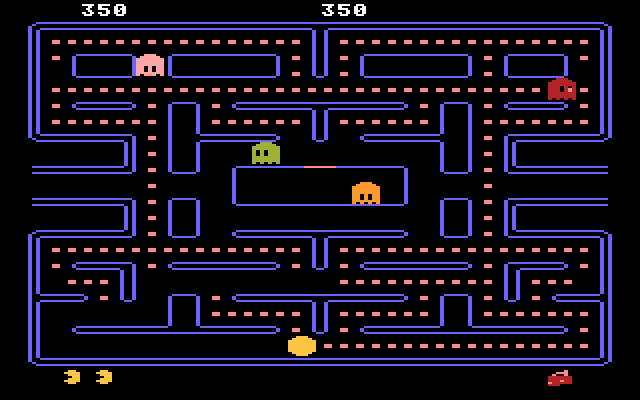
\includegraphics[scale = 0.3]{PacMan_Original}
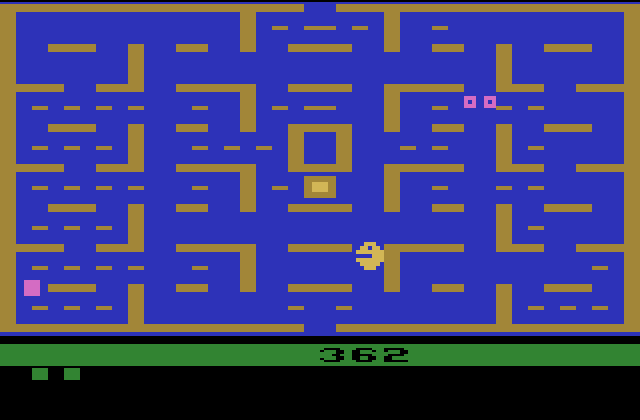
\includegraphics[scale = 0.285]{PacMan_(1982)_Atari_Port}{
    \emph{PacMan} on the Atari 5200 (left), compared to the famously poor Atari 2600 port (right).
}




When Blitworks faced porting 'Fez' to the Playstation 3 the most difficult challenge they had was that the original Fez game was written in C\#, and there was no C\# support for PlayStation platforms when they started the port, so they faced the big decision of trying to port the whole Mono runtime or to convert the game to C++ \cite {gamasutra2014}.

 Some have chosen to restrict access as much as possible, whereas others have chosen to disclose the entire source code of their SDK and OS \cite {holzer2009trends}.


\section*{Hardware}

Greatly differing or inadequate resources on the target platform are the cause of many failed ports. Despite the PS3 being the most technologically advanced video game console of the seventh generation \cite {ofek2008sony}, developing required a lot of effort, source code developed for the CELL processor is not portable at all on other architectures \cite {buttari2007limitations}, so developers would concentrate on the Xbox 360 and port to the ps3 later.  Bayonetta suffered famously from this port, with load times between levels far longer than the original \cite {Kotaku2010Bayonetta}.



